	\author{Jakub Pietrucha}
\title{CV}

\documentclass{report}
\usepackage{graphicx}
\usepackage{multirow}
\usepackage{array}
\linespread{1.5}
\textwidth17cm
\oddsidemargin0cm
\hoffset0cm

\begin{document}
\def\thesection{}
\def\thepage{}
\def\thefootnote{}
\begin{center}
	\textbf{\Large{Jakub Pietrucha}}
	\vspace{0.3cm}
\end{center}

\begin{tabular}{p{2.5cm}|p{9cm} r} 
Birth date    & \ 17.08.1986 &\multirow{3}{*}{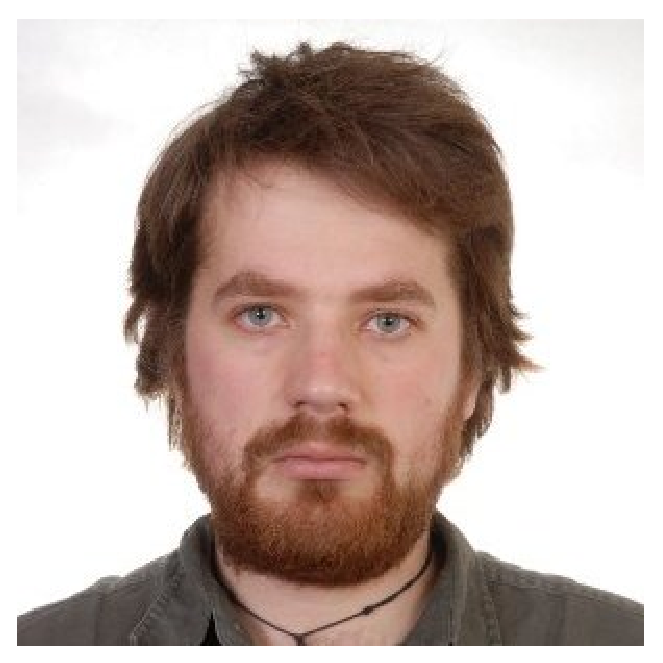
\includegraphics[width=20mm]{photo.eps}} 	\\
Marital status& \ married\\
Phone number  & \ +48 511 927 646\\
E-mail        & \ jakub.pietrucha@gmail.com \\
\end{tabular} 

\section{Employment History}
\begin{tabular}{p{5cm} p{10cm}}
\textbf{08.14--07.15} &\textbf{Intel}\\
\hline
Research consultant in project XMM7360, FEFC
&Participating in the project through whole release cycle. Hands-on experience in majority of component features. Designing and developing FEFC test environment using SystemC API. Hunting down software and hardware bugs during product bring-up. \\
\textbf{05.13--07.14} &\textbf{Nokia}\\
\hline
Senior DSP Software Specialist in project ULPHY, LTE eNB
&Implementing parts of MU-MIMO, three component carrier aggregation and channel estimation in PUSCH. Configuring boost library for Texas Instruments compiler. Building team spirit and preaching the word of scrum. Organizing Coding Dojo. Exploring the rims of pair programming and TDD.\\
\textbf{17.10--04.13} &\textbf{Nokia}\\
\hline
DSP software engineer in project ULPHY, LTE eNB
&Designing and implementing software for LTE eNodeB, physical layer. Focused on algorithms design and optimizations. Working with Physical Random Access Channel and Physical Uplink Control Channel.\\
\textbf{05.08--09.08; 10.08--11.08} &\textbf{Advanced LED systems}\\
\hline
Application engineer
&Designing linear and switching LED drivers. Assembling and
testing prototypes. Preparing technical documentation.
\end{tabular}

\section{Education}
	\begin{tabular}{m{1.4cm} m{2.3cm} m{2.4cm} m{2.8cm} m{4.6cm}}
	&\begin{center}	\textbf{Institution} \end{center}
	&\begin{center} \textbf{Faculty} \end{center} 
	&\begin{center}	\textbf{Major} \end{center} 
	&\begin{center}	\textbf{Thesis Title}  \end{center}\\
	\hline
	\begin{center} 10.07.2010 \end{center}
	&\begin{center}	Wroclaw University\linebreak[4] of Technology	\end{center} 
	&\begin{center}	Faculty of \linebreak[4] Microsystems Electronics and Photonics	\end{center} 
	&\begin{center}	Electronics and Telecommunication	\end{center}
	&\begin{center}	New algorithms of analysis of high resolution X-ray diffraction measurements data in the NSCA software	\end{center}\\ 
	\begin{center} 13.02.2013 \end{center}
	&\begin{center}	Wroclaw University\linebreak[4] of Technology	\end{center} 
	&\begin{center}	Faculty of \linebreak[4] Fundamental Problems of Technology	\end{center} 
	&\begin{center}	Physics	\end{center}
	&\begin{center}	Not conferred \end{center}\\
	\end{tabular}

\section{Languages}
\begin{tabular}{ccc}
	&Spoken &Written\\
	\hline	 
	English &proficient &proficient\\
	Polish &native &native\\
\end{tabular}

\section{Interests}
traveling,  hiking, canoing, cooking, board games
\footnote{I agree to the processing of the personal data included in my application for the purposes of the recruitment process}
\end{document}